\chapter{Placement}
The algorithm for the placement, a deterministic analog circuit placement algorithm using hierarchically bounded enumeration and enhanced shape functions \cite{iccad:plantage}, was mainly developed and implemented by Martin Strasser in his doctoral thesis as well as by Michael Eick during his diploma thesis. The main idea behind it is that circuits typically have a certain hierarchy. For example, an operation amplifier \figref{fig:miller_amplifier_schematic} consists of a differential amplifier, a current mirror and an output amplifier. Usually it is a good idea to place the modules of the same group not too far away because they belong together in the functionality of the circuit. This is also the typical way a designer creates a layout out of a circuit manually. The designer starts with a certain functionality and places the modules for this function close to each other. If the modules are grouped together in the layout \figref{fig:miller_amplifier_layout}, they do not see that large differences in, for example, temperature of the substrate. This will result in a better performance of the circuit.
At the moment, this information on the groups must be fed in by the user but the target for the future would be that even this step could be automatized by, for instance, a circuit analysis. Consequently, the information can be used to find the best placements for these groups, which are then combined on the next level in the hierarchy.

\begin{figure}	
	\centering	
	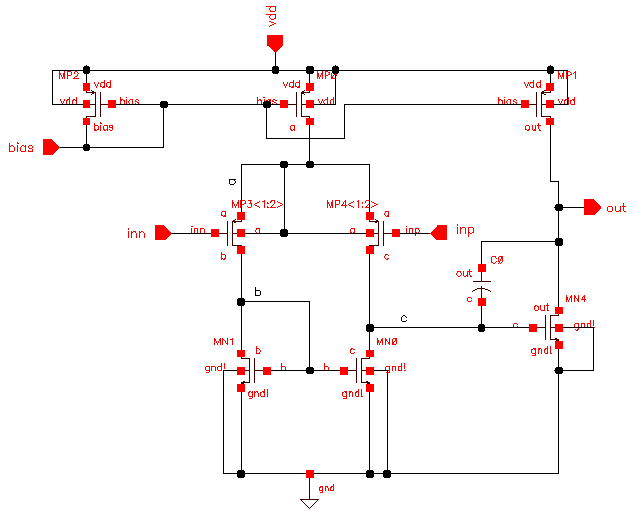
\includegraphics[scale=0.6]{FIG/miller_amplifier_schematic.png}	
	\caption{schematic of a miller amplifier}	
	\label{fig:miller_amplifier_schematic}
\end{figure}

\begin{figure}
	\centering
	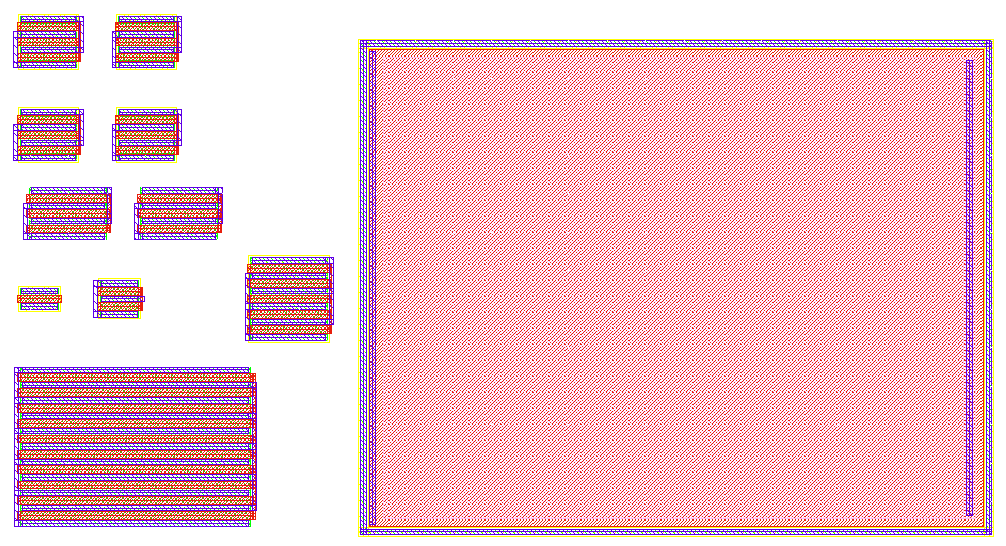
\includegraphics[scale=0.4]{FIG/miller_amplifier_layout.png}
	\caption{possible layout for a miller amplifier}
	\label{fig:miller_amplifier_layout}
\end{figure}

Additionally, it is possible to define certain constraints for modules and groups of modules:
\begin{itemize}
\item symmetry
\item alignment
\item group symmetry
\item group alignment
\item same variants
\end{itemize}

Some of these have to be considered by the routing, because, for example, symmetric modules typically should also have symmetric routes to avoid different resistances of the routes. Furthermore, if examined in more detail, symmetric routes should even have similar capacitive couplings with other routes.

The general structure of this application is divided into two parts:
\begin{itemize}
\item ICFBInterface
\item Plantage
\end{itemize}

First, I will start with a short description of Plantage. It is a simple command line tool which accepts an XML-input-file and produces an XML-output-file. The input-file contains the basic information on the circuit, e.g. the modules with their various variants, group definitions, constraints and so on. The output-file of this tool contains a so-called \emph{shape function} with different shapes. The shapes are the actual placements which contain the positions of the modules and the selected variants.

The ICFBInterface is, as its name already suggests, an interface between Cadence and Plantage. It receives, for example, the data of a circuit from Cadence. Based on this data, the users has to define groups and constraints, where the ICFBInterface supports them. This information is then sent to Plantage, which calculates several possible layouts. These layouts are returned in form of a shape function back to the ICFBInterface. There the results are displayed and the user can generate layouts in Cadence.

\section{Algorithm}
As already mentioned before, the placement is generated hierarchically. The starting point for the calculation of a placement is an enumeration sequence. This value is a very compact way to store the information of related positions for an accumulation of modules. It consists of a list of Boolean variables, usually stored as a string with the values \textit{E} for East and \textit{N} for North. The modules and selected variants for this enumeration are then stored in a B*-tree. On this data structure the actual calculation of the coordinates, considering the given constraints, is done. From the B*-tree several lines for a linear program are created. After this the linear program is solved by an external application, at the moment lp\textunderscore solve \cite{lp_solve}. This tool solves the linear program and from the solution the actual coordinates for the modules can be calculated. This is usually done for some different enumerations. The list of possible placements, which is generated that way, is then filtered by the area. To reduce the computing time only a certain number of placements is then used on the next higher hierarchy level.

\section{Software Architecture}
In the following part only the software architecture of Plantage will be described, as this was the main part for the implementation of the routing. On the side of the GUI only some additional information needed to be displayed or manipulated by the user.

Plantage is a typical example for a grown code base. It contained a lot of different coding styles, had some half-implemented features and a lot of old and dead development branches, which were part of the production code. So my first task was to eradicate parts that were not in use anymore and unify the code base. The main problem was that the existing and working features should not be broken, what could have happened easily. For the beginning, I generated some test inputs, which covered the most important features. After every risky change I could generate the output from this data and compare it with the results before each change. Through this practise I was able to slowly refactor the code and increase the encapsulation for some parts. This enabled me to write unit tests for these parts and reduce the risk of broken features even more. One by one, I applied this to nearly the complete code base. The result of these steps is a now well-tested and -documented code base, which can be changed and improved easily. Additionally, the basic structure of the architecture improved, or better said, an architecture was developed and applied to the code. Therefore, it became easier to understand what the different parts of the code actually do. This was also important for the implementation of a routing algorithm, as it also produced a single point, where the routing can be done.